\section{Initial System Designs}
\label{sec:isd}
\subsection{Route Discovery/Landing Page}
\begin{figure}[!ht]
    \begin{center}
        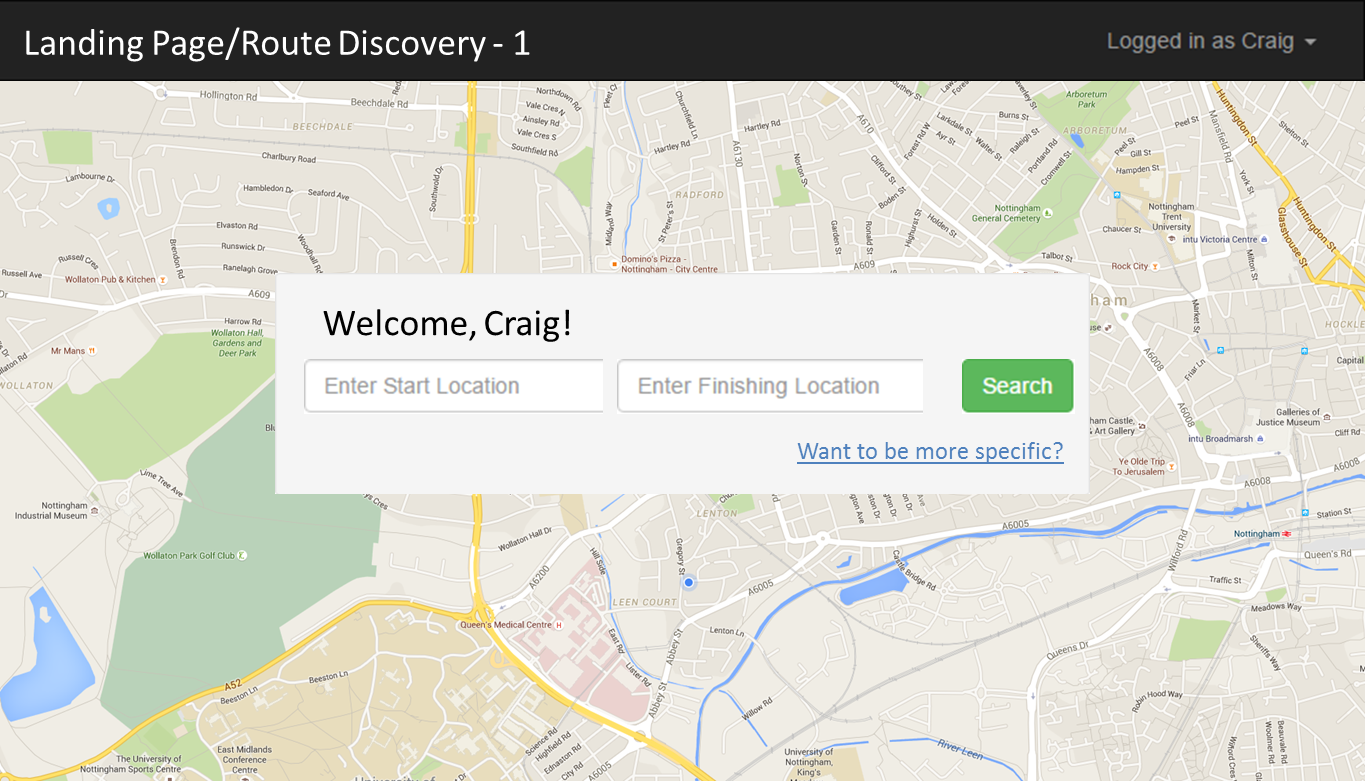
\includegraphics[width=0.725\textwidth]{images/appendix/landing1.png}
    \end{center}
    \vspace{-6mm}
\end{figure}

\begin{figure}[!ht]
    \begin{center}
        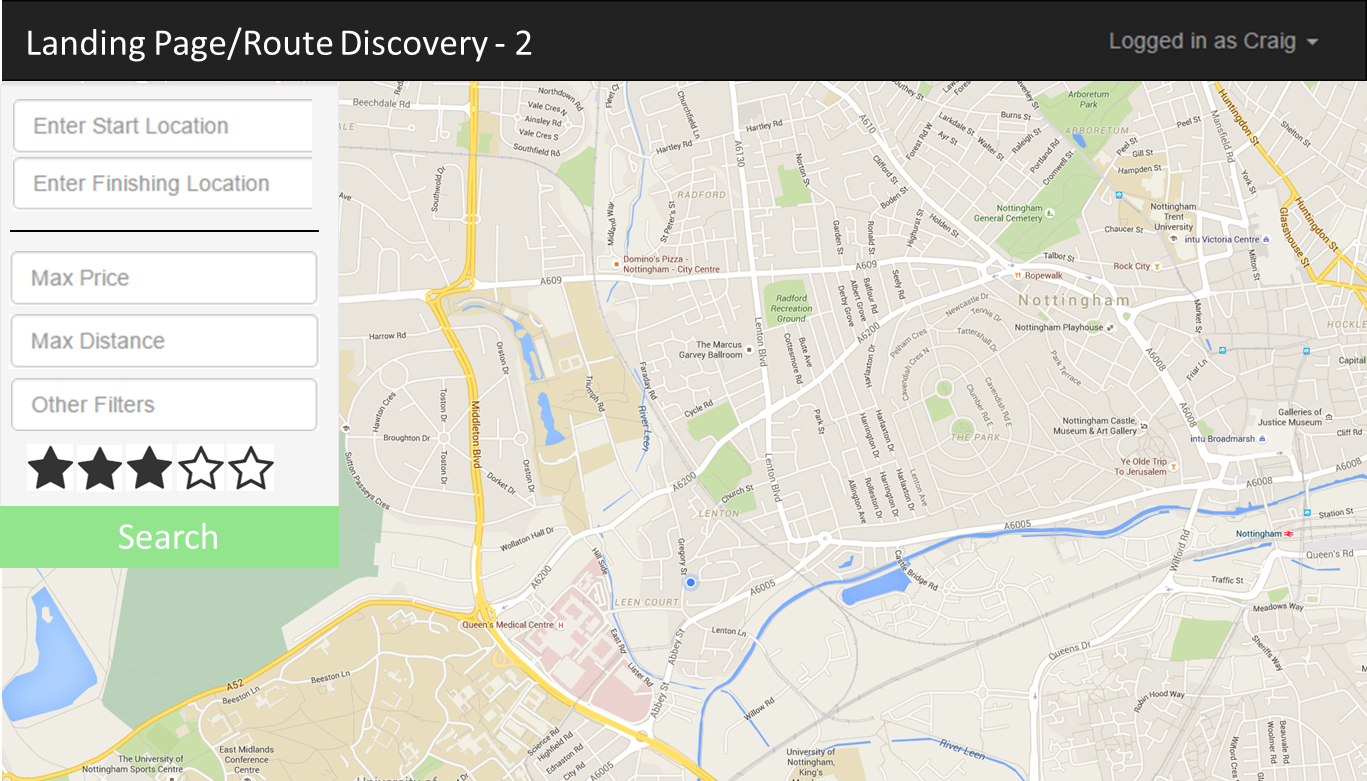
\includegraphics[width=0.725\textwidth]{images/appendix/landing2.png}
    \end{center}
    \vspace{-6mm}
\end{figure}

\begin{figure}[!ht]
    \begin{center}
        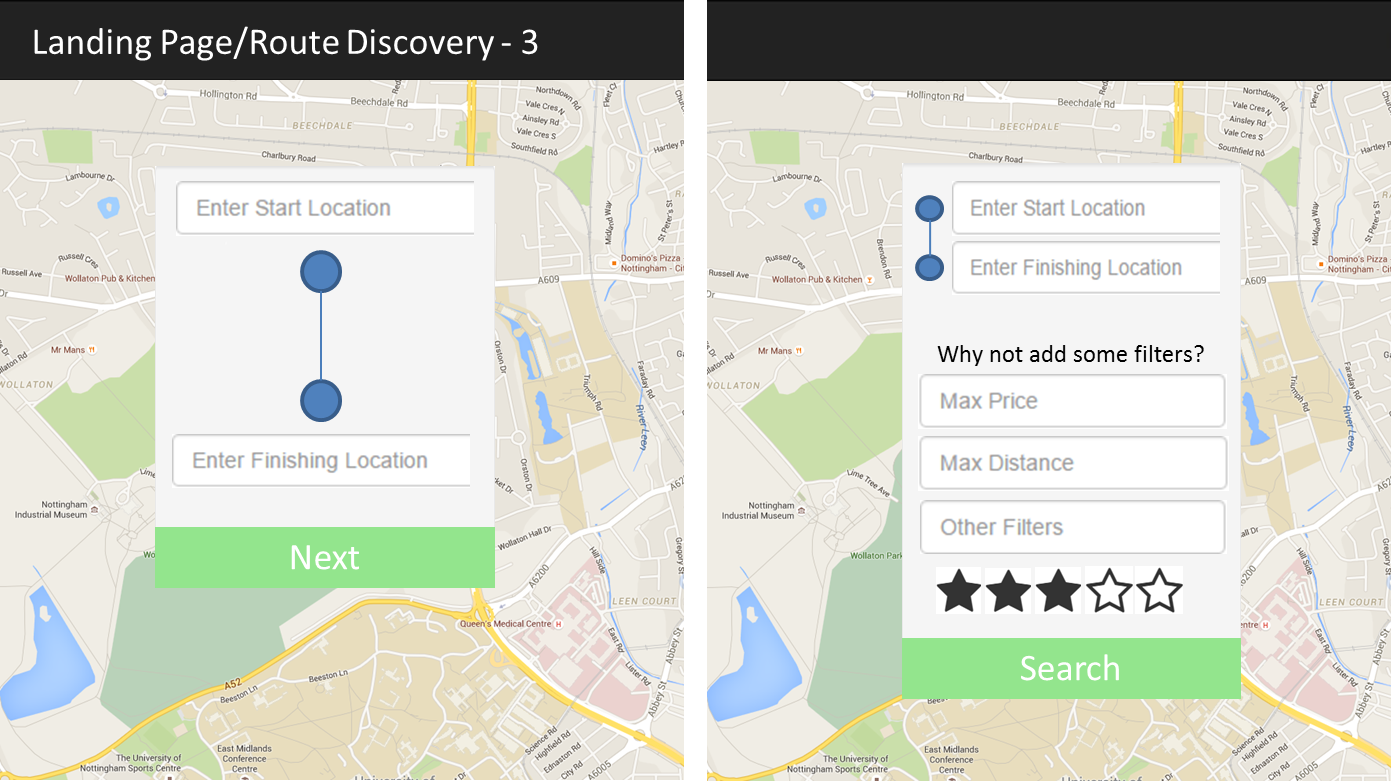
\includegraphics[width=0.725\textwidth]{images/appendix/landing3.png}
    \end{center}
    \vspace{-6mm}
\end{figure}

\newpage 
\subsection{Route Listing Page}
\begin{figure}[!ht]
    \begin{center}
        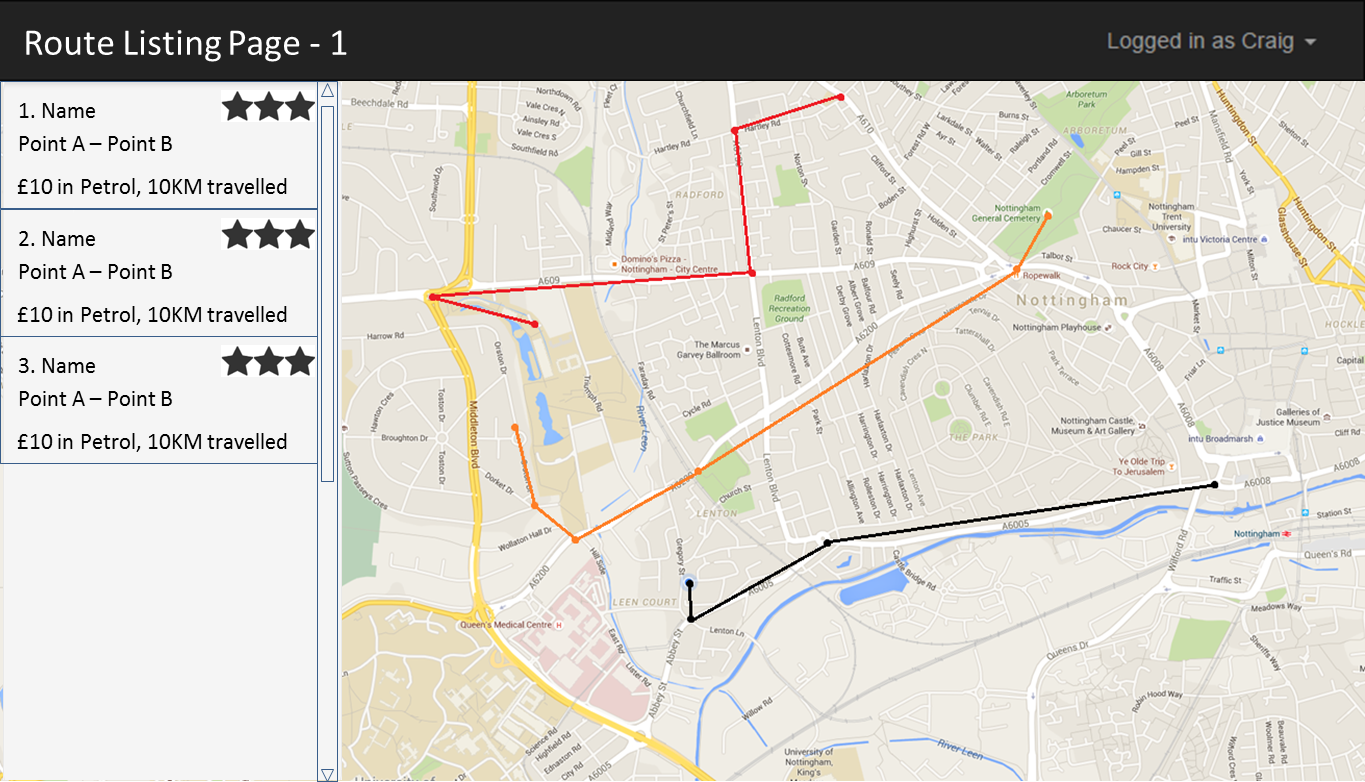
\includegraphics[width=0.75\textwidth]{images/appendix/rlp1.png}
    \end{center}
    \vspace{-6mm}
\end{figure}

\begin{figure}[!ht]
    \begin{center}
        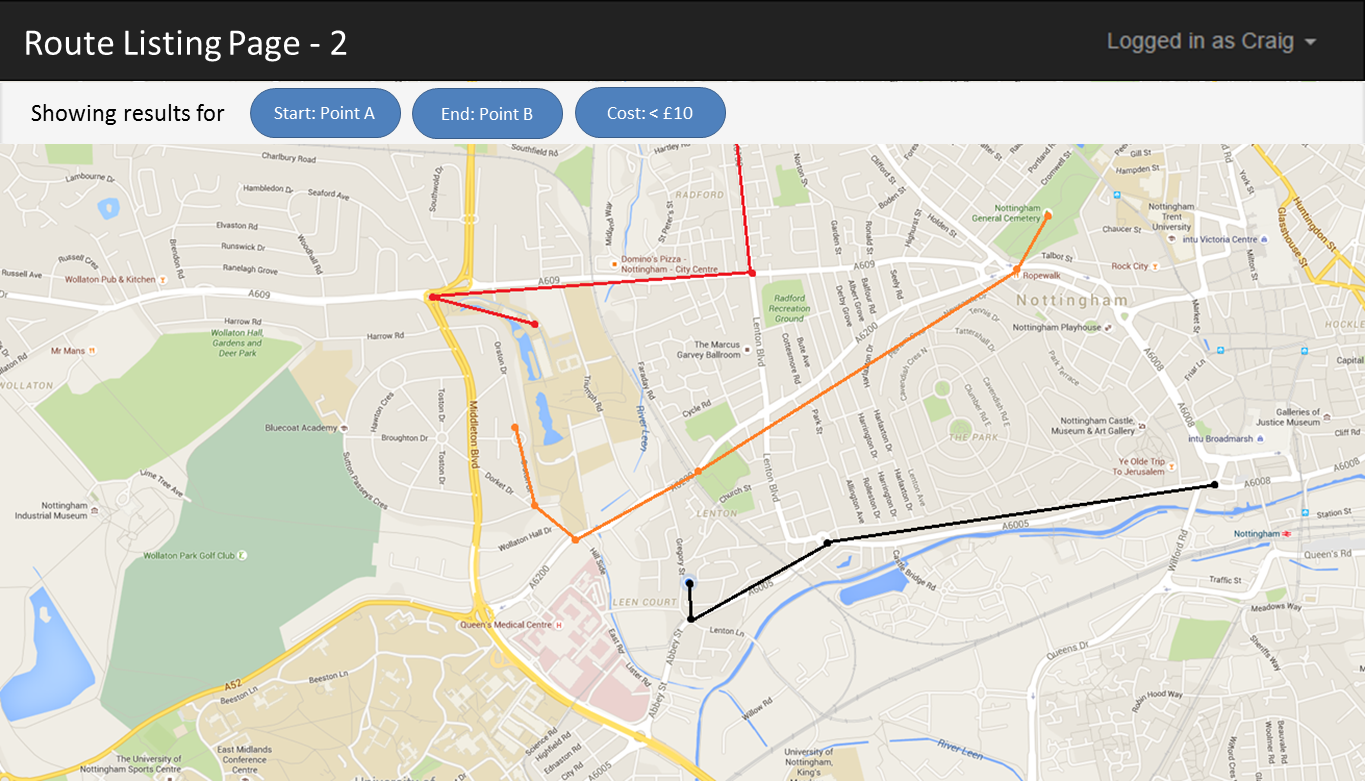
\includegraphics[width=0.75\textwidth]{images/appendix/rlp2.png}
    \end{center}
    \vspace{-6mm}
\end{figure}

\begin{figure}[!ht]
    \begin{center}
        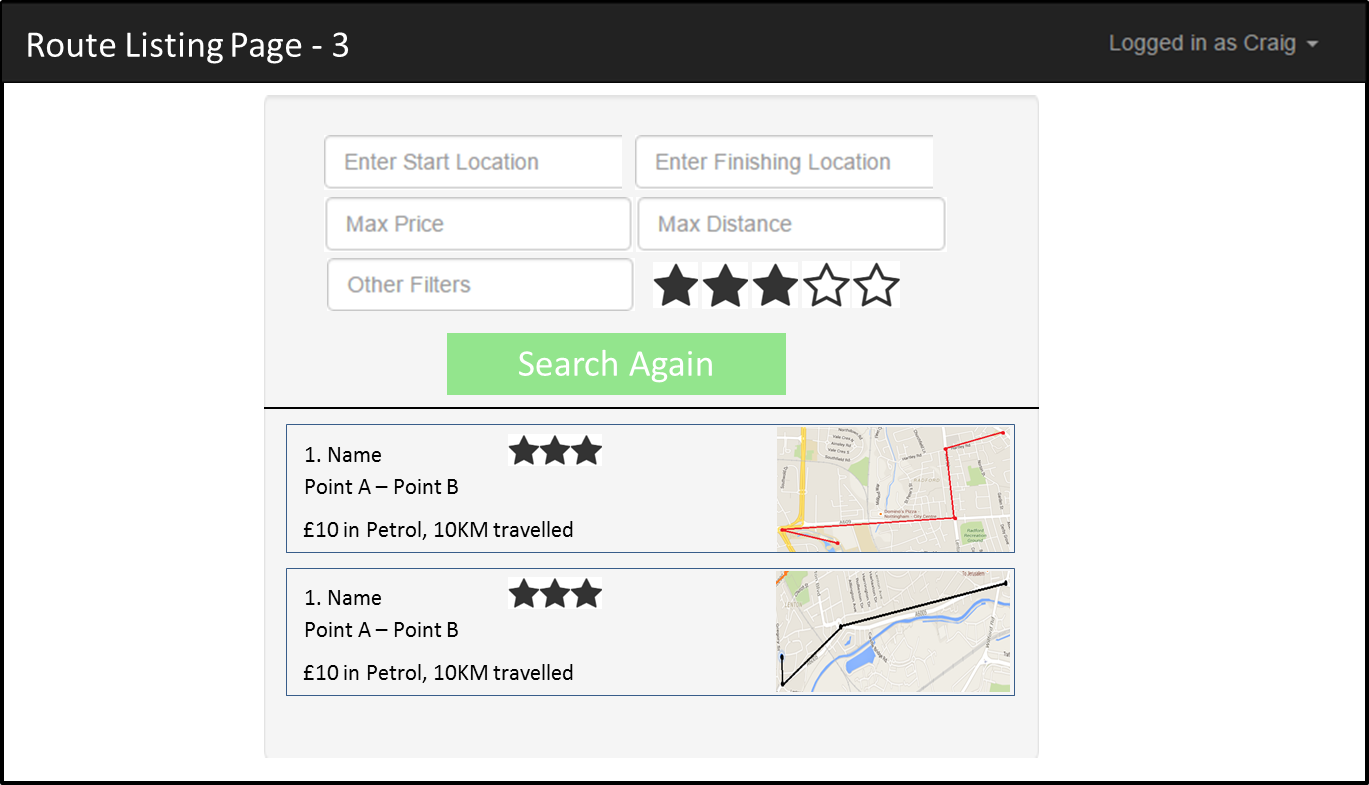
\includegraphics[width=0.75\textwidth]{images/appendix/rlp3.png}
    \end{center}
    \vspace{-6mm}
\end{figure}

\newpage 
\subsection{Route Detail Page}
\begin{figure}[!ht]
    \begin{center}
        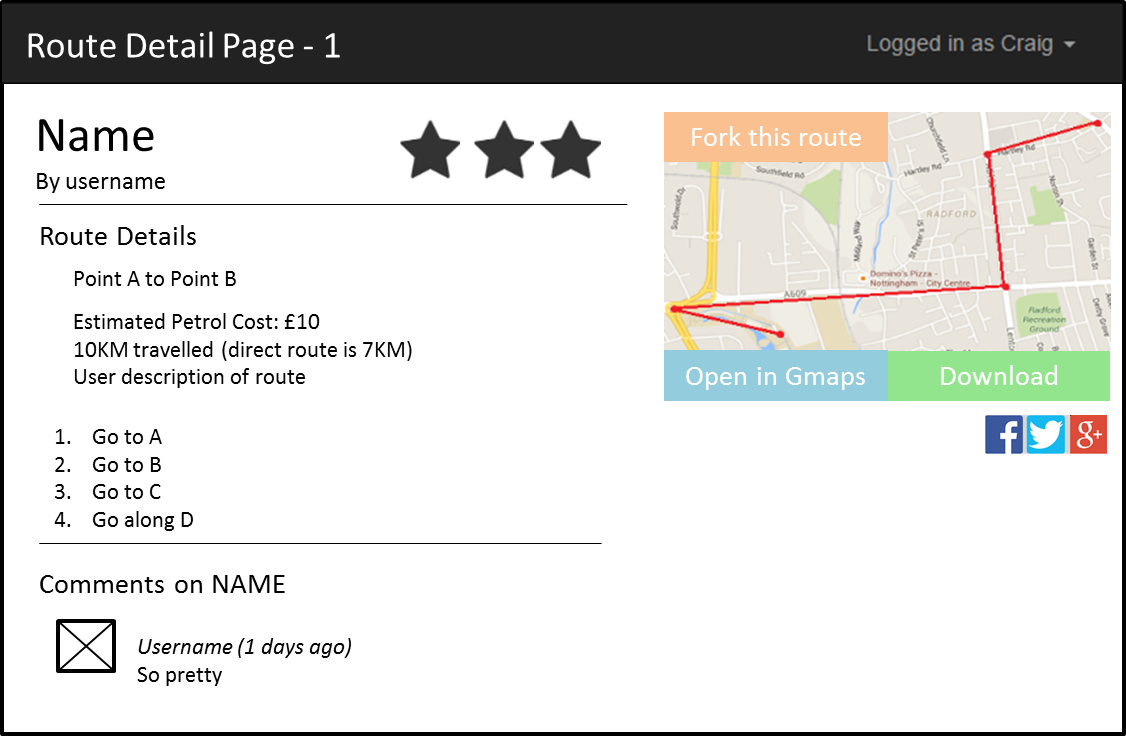
\includegraphics[width=0.75\textwidth]{images/appendix/rdp1.png}
    \end{center}
    \vspace{-6mm}
\end{figure}

\begin{figure}[!ht]
    \begin{center}
        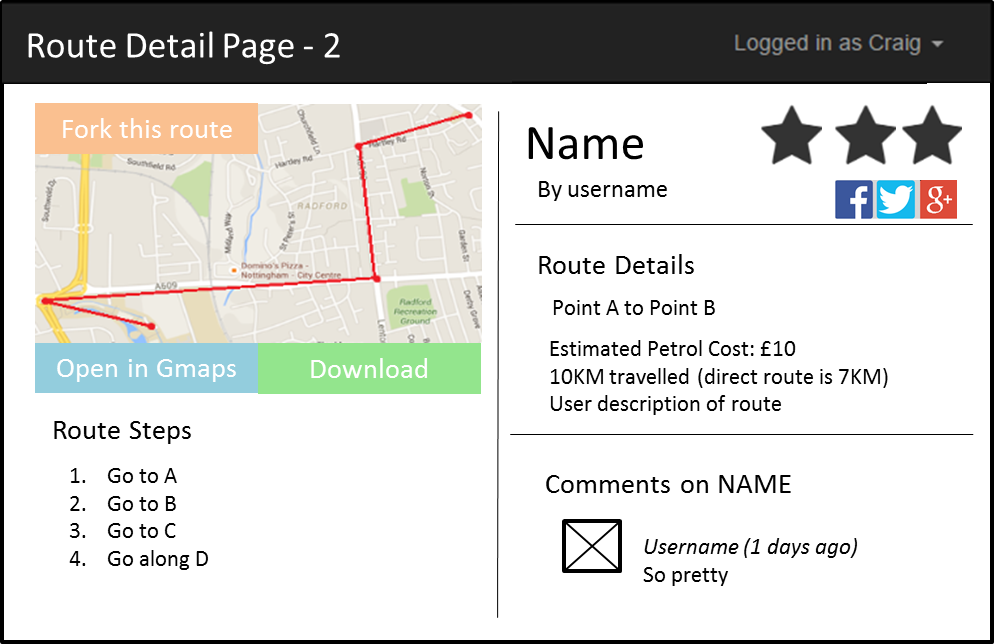
\includegraphics[width=0.75\textwidth]{images/appendix/rdp2.png}
    \end{center}
    \vspace{-6mm}
\end{figure}

\begin{figure}[!ht]
    \begin{center}
        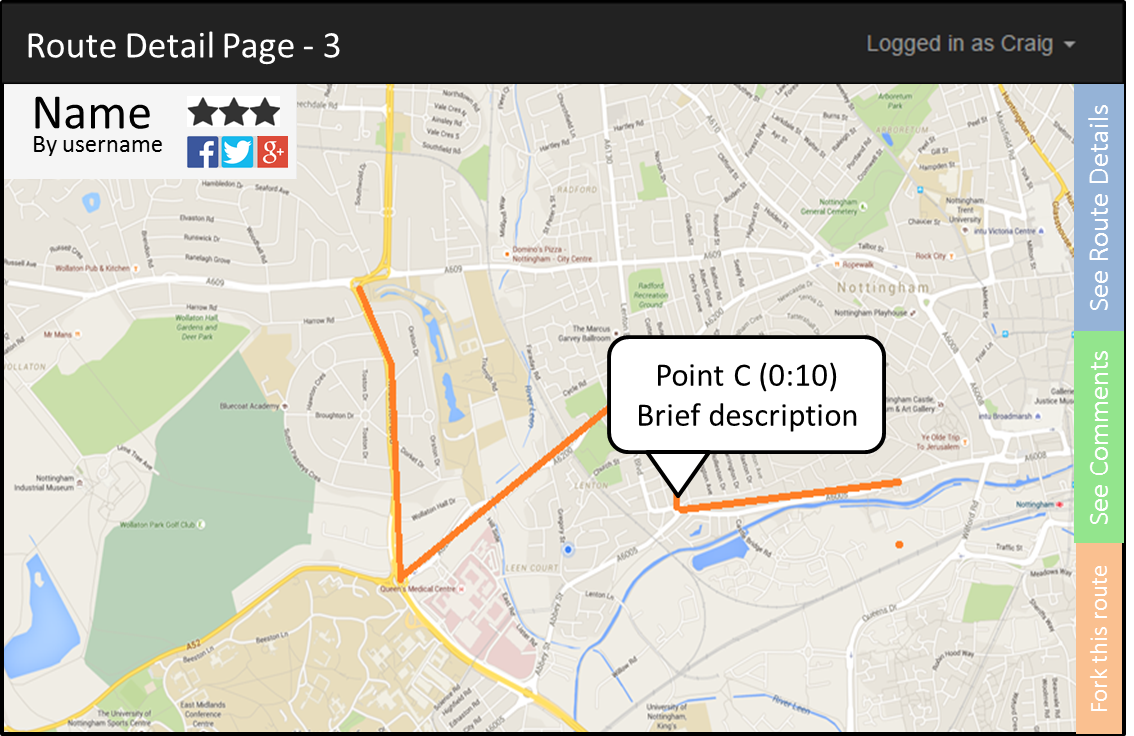
\includegraphics[width=0.75\textwidth]{images/appendix/rdp3.png}
    \end{center}
    \vspace{-6mm}
\end{figure}

\subsection{Route Creation Page}
\begin{figure}[!ht]
    \begin{center}
        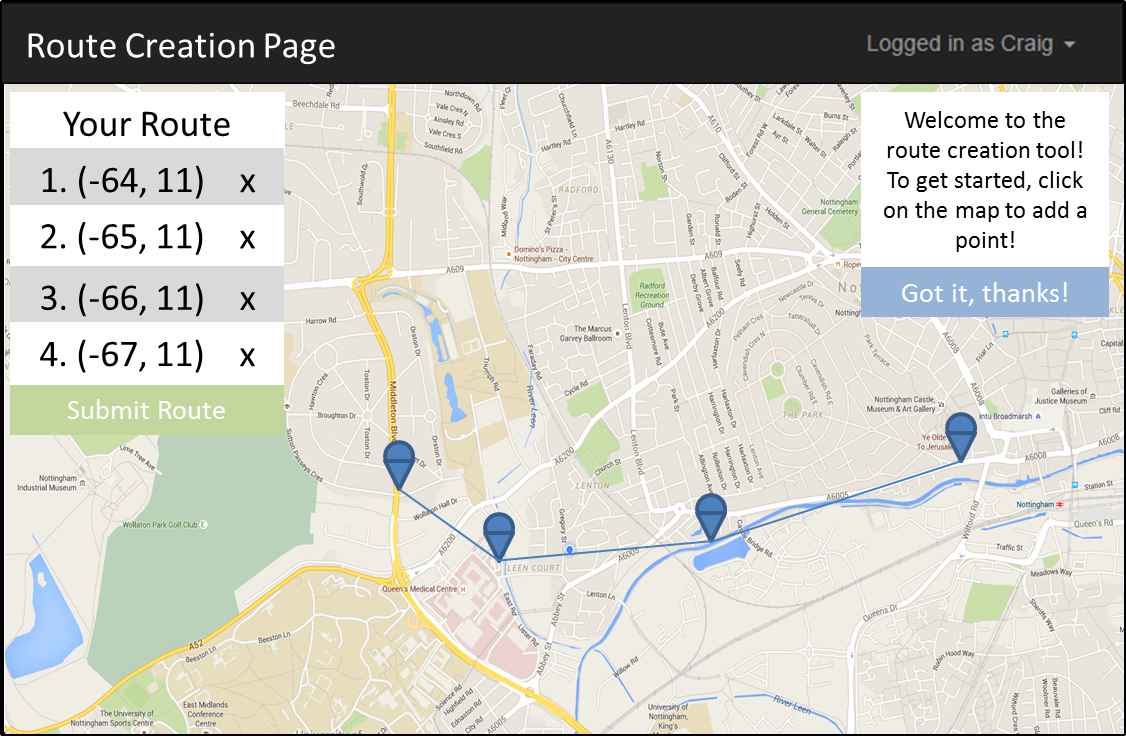
\includegraphics[width=0.8\textwidth]{images/appendix/rcp1.png}
    \end{center}
    \vspace{-6mm}
\end{figure}

\subsection{Profile Page}
\begin{figure}[!ht]
    \begin{center}
        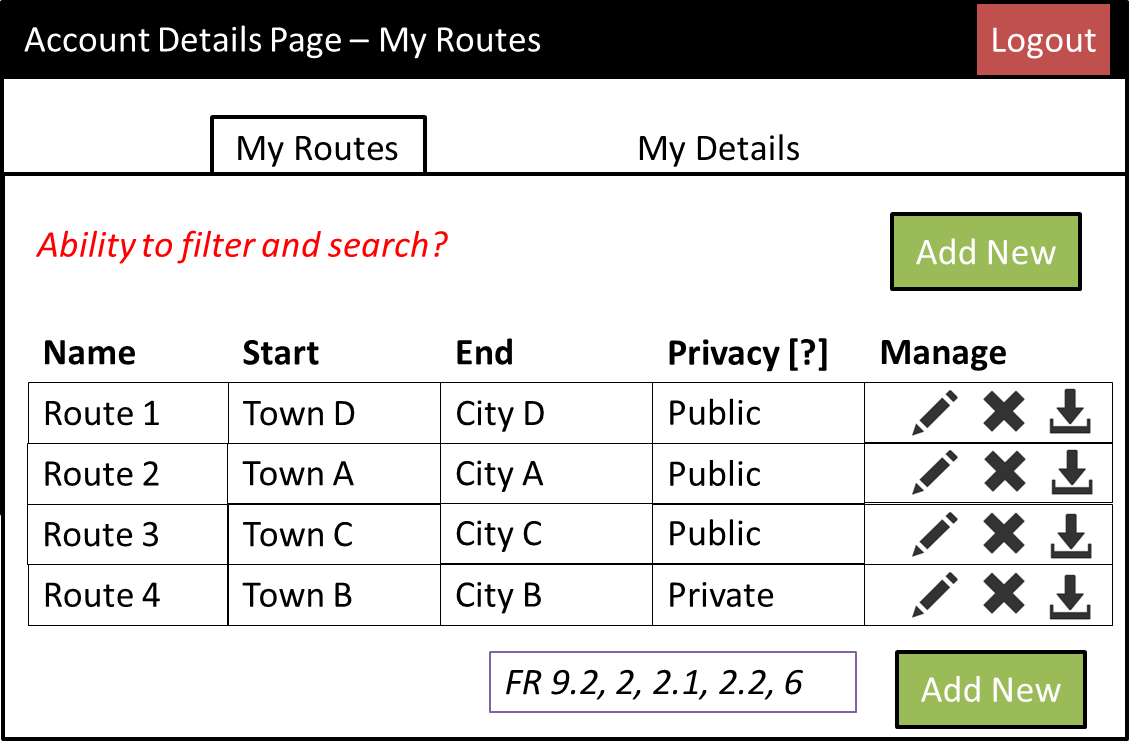
\includegraphics[width=0.8\textwidth]{images/appendix/prof1.png}
    \end{center}
    \vspace{-6mm}
\end{figure}


\newpage 
\section{Interface Design Heuristics}
\label{sec:idh}

\subsection{Jakob Nielsen's Usability Heuristics}
\begin{enumerate}
    \item Visibility of system status
    \item Match between system and the real world
    \item User control and freedom
    \item Consistency and standards
    \item Error prevention
    \item Recognition rather than recall
    \item Flexibility and efficiency of use
    \item Aesthetic and minimalist design
    \item Help users recognize, diagnose, and recover from errors
    \item Help and documentation
\end{enumerate}

\subsection{Ben Schneiderman's Golden Rules}
\begin{enumerate}
    \item Strive for consistency.
    \item Enable frequent users to use shortcuts.
    \item Offer informative feedback.
    \item Design dialog to yield closure.
    \item Offer simple error handling.
    \item Permit easy reversal of actions.
    \item Support internal locus of control.
    \item Reduce short-term memory load.
\end{enumerate}


\newpage 
\newgeometry{left=15pt,right=20pt,top=30pt,bottom=20pt}
\pagestyle{none}
\begin{landscape}
\section{Project Gantt Chart}
\label{sec:gantt}
	\begin{center}
		\begin{ganttchart}[
			y unit chart = 0.6cm,
			y unit title = 0.6cm,
			x unit = 0.6cm,
			vgrid,
			hgrid,
			Mile1/.style={milestone/.append style={fill=green}},
			Mile2/.style={milestone/.append style={fill=red}}
			]{1}{32}
			\gantttitle{Project Time Plan}{32}\\ 
			\gantttitlelist{"Oct"}{4}
			\gantttitlelist{"Nov"}{5}		
			\gantttitlelist{"Dec"}{4}	
			\gantttitlelist{"Jan"}{4}
			\gantttitlelist{"Feb"}{5}
			\gantttitlelist{"Mar"}{4}			
			\gantttitlelist{"Apr"}{4}	
			\gantttitlelist{"May"}{2}\\
			\gantttitlelist{5, 12, 19, 26,
				2, 9, 16, 23, 30,
				7, 14, 21, 28,
				4, 11, 18, 25,
				1, 8, 15, 22, 29,
				7, 14, 21, 28,
				4, 11, 18, 25,
				2, 9
			}{1}\\
			\ganttset{progress label text={},
				bar incomplete/.append style={fill=green!40},
				group/.append style={draw=black, fill=green},}
			\ganttgroup{Documentation}{1}{28} \\
			\ganttbar[progress=0]{1. Design Specification}{1}{1}\\ 					%0
			\ganttbar[progress=0]{2. Initial Project Plan}{2}{2}\\						%1
			\ganttmilestone[Mile1]{Initial Project Plan Deadline (17th)}{2}\\	%2	
			\ganttbar[progress=0]{3. Revised Project Plan}{4}{4}\\						%4
			\ganttmilestone[Mile1]{Revised Project Plan Deadline (2nd)}{4}\\	%5				
			\ganttbar[progress=0]{4. Write Dissertation}{25}{28}\\						%17
			\ganttmilestone[Mile1]{Hand-in Dissertation (18th)}{28}\\			%18

			\ganttset{progress label text={},
				bar incomplete/.append style={fill=blue!40},
				group/.append style={draw=black, fill=blue},}
			\ganttgroup{Development}{5}{23} \\											
			\ganttbar[progress=0]{5. Sign Up Page (A1, O4)}{5}{5}\\								%6
			\ganttbar[progress=0]{6. Log In Page (A1, O2)}{5}{5}\\								%7
			\ganttbar[progress=0]{7. My Details Page (O4)}{5}{5}\\							%8
			\ganttbar[progress=0]{8. Route Creation Page (O2)}{6}{7}\\						%9
			\ganttbar[progress=0]{9. My Routes Page (O4)}{9}{9}\\							%13
			\ganttbar[progress=0]{10. Route Detail Page (O3, O6)}{10}{11}\\						%14
			\ganttbar[progress=0]{11. Route Discovery Page (O1)}{17}{18}\\					%13
			\ganttbar[progress=0]{12. Route Listing Page (O1)}{19}{20}\\						%15
			\ganttbar[progress=0]{13. Admin Page and Functionality (O5)}{21}{23}\\			%16
		
			\ganttset{progress label text={},
						bar incomplete/.append style={fill=red!40},
						group/.append style={draw=black, fill=red},}
			\ganttgroup{Misc. Tasks}{3}{31} \\						
			\ganttbar[progress=0]{14. Set up database structure}{3}{3}\\				%3
			\ganttbar[progress=0]{15. Set up web hosting and repository}{3}{3}\\		
			\ganttbar[progress=0]{16. Add Test Routes}{8}{8}\\							%11			
			\ganttbar[progress=0]{17. Prepare for demonstration}{30}{31}\\				%19	
			\ganttmilestone[Mile2]{Demonstration (3rd-5th)}{31}\\				%20
					
		\ganttset{progress label text={},
			bar incomplete/.append style={fill=purple!40},
			group/.append style={draw=black, fill=purple},}
		\ganttgroup{Other Commitments}{6}{16} \\											
		\ganttbar[progress=0]{18. Other Coursework Deadlines}{6}{8}\\	
		\ganttbar[progress=0]{19. Exam Revision/Final Courseworks}{11}{16}\\		%14    
	\end{ganttchart}
	\end{center}
\end{landscape}

\newpage
\restoregeometry
\newgeometry{left=3cm, right=3cm, top = 75pt, bottom=75pt}
\pagestyle{appendix}


